\chapter{QAM信号量子接收机}
在上一章中,我们回顾了现有的一些量子接收机实现方案,
包括二元检测和多元的PSK和PPM检测量子接收机。
但是到目前为止,专门针对QAM信号设计的量子接收机
研究还比较少。然而,QAM信号具有很高的频谱效率,
已被应用到大容量光通信系统之中\cite{winzer2012high}。
因此,研究QAM信号量子接收机是一件很有必要的事情。

\section{QAM信号接收机理论极限}
\subsection{标准量子极限}
在经典通信系统中,常用外差接收机检测QAM信号,
这种接收机的性能也叫QAM信号的标准量子极限(SQL)\cite{kato1999quantum}。
设$M$阶QAM信号由$M$个相干态构成,如图\ref{fig:QAM-signals}所示,
显示的是16-QAM和36-QAM星座图。假设$M$阶QAM信号每一个
正交幅度$X$或$P$都可以取$L$个不同的值,那么$M=L^2, L=3,4,5...$。
设这$L$元基本符号集合为
\begin{equation}
\Omega = \{-(L-1) + 2(i-1) | i=1,2,...,L\}.
\label{eq:QAM-omega}
\end{equation}
那么$M$阶QAM信号
可以表示为
\begin{equation}
\ket{\alpha_{uv}} = \ket{\alpha(u + j v)}, (u, v) \in \Omega. 
\end{equation}
这里$j=\sqrt{-1}$。例如,16-QAM信号就可以用相干态表示为
\begin{equation}
\begin{split}
\ket{\alpha_{1,1}} &= \ket{\alpha(1 + j )}, \\
\ket{\alpha_{1,3}} &= \ket{\alpha(1 + j 3)}, \\
\ket{\alpha_{1,-1}} &= \ket{\alpha(1 - j )}, \\
                &\vdots                      \\
\ket{\alpha_{-3,-3}} &= \ket{\alpha(-3 - j 3)}.
\end{split}
\end{equation}
这里取$\alpha > 0$,那么M阶QAM信号信号平均光子数为
\begin{equation}
\begin{split}
n &= |\alpha|^2 \frac{1}{M}\sum_{u \in \Omega}\sum_{v \in \Omega} (u^2+v^2)\\
  &= \frac{2}{3}(M-1) |\alpha|^2.
\end{split}
\end{equation}


\begin{figure}
\centering
  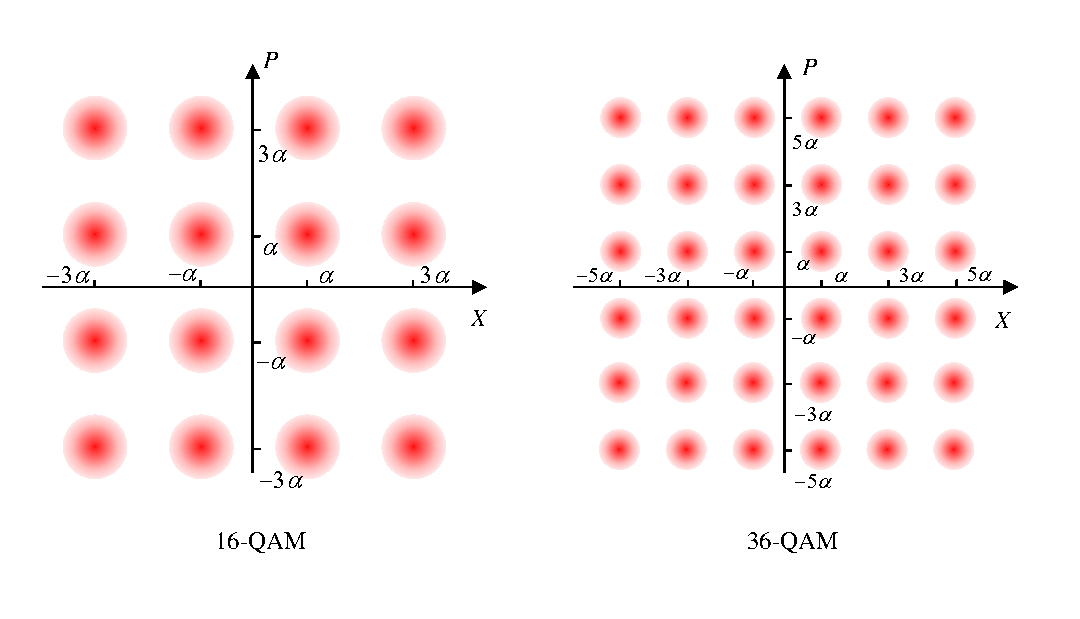
\includegraphics[width=0.8\textwidth]{figures/chap3/QAM-signals}
  \caption{QAM信号星座图}
  \label{fig:QAM-signals}
\end{figure}


下面我们来计算一下QAM信号的标准量子极限。
利用式\ref{eq:Her-receiver-output}可得理想情况下,
外差接收机的概率密度函数为\cite{kato1999quantum}
\begin{equation}
p(x_c, x_s| u, v) = \frac{1}{\pi} \exp[-(x_c - u\alpha)^2 - (x_s - v\alpha)^2]
\end{equation}
这里$x_c$和$x_s$对应于式\ref{eq:Her-receiver-output}中的$\alpha_1$和$\alpha_2$,
是接收机输出的两个正交幅度观测量。
根据贝叶斯检测理论,最优判决区域为
\begin{equation}
D_{u',v'} = \{ (x_c,x_s)| D_L(u')\alpha < x_c \le D_U(u')\alpha,  D_L(v')\alpha < x_s \le D_U(v')\alpha \}
\end{equation}
这里$D_U$和$D_L$是两个上下界函数,对给定的参数$L$,
定义为
\begin{equation}
\begin{split}
D_L(u) &= \begin{cases}    
          -\infty     & u < -(L-2)  \\
          (u-1) & otherwise
         \end{cases}\\
D_U(u) &= \begin{cases} 
          \infty     & u > L-2  \\
          (u+1) & otherwise
         \end{cases}
\label{eq:LU-fun}
\end{split}
\end{equation}
即将复平面划分成如图\ref{fig:QAM-domain-split}所示的$M$个判决
区域,将输出统计量落在某个区域的结果判决为在该区域内的符号。
那么,外差接收机的平均错误概率为
\begin{equation}
\begin{split}
P_e &= 1 - \frac{1}{M} \sum_{u\in\Omega}\sum_{v\in\Omega} \iint_{D_{u,v}} p(x_c,x_s|u,v) dx_c dx_s \\
    &= 1 - \frac{1}{M}[1+(L-1) \erf(\alpha)]^2.
\end{split}
\end{equation}
因此,当平均光子数很大时,即$|\alpha|^2 \gg 1$,
利用余误差函数的Chernoff界\cite{chang2011chernoff},
可得QAM信号外差接收机的渐近性能为
\begin{equation}
\begin{split}
P_e &\approx 2(1 - \frac{1}{L}) e^{-\alpha^2}.
\label{eq:QAM-SQL-approx}
\end{split}
\end{equation}

\begin{figure}
\centering
  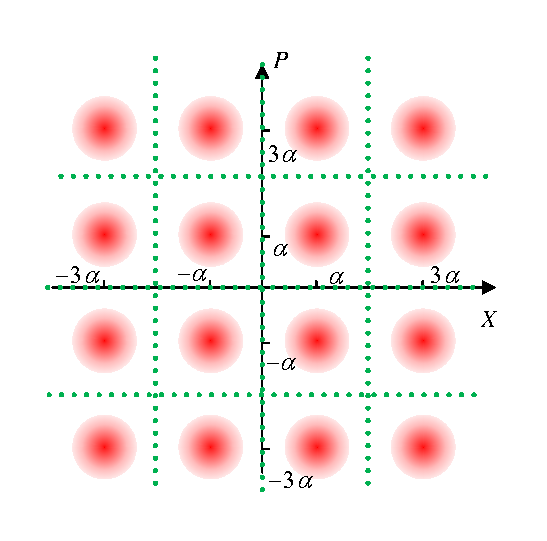
\includegraphics[height=5cm]{figures/chap3/QAM-domain-split}
  \caption{16-QAM信号外差接收判决区域划分示意图}
  \label{fig:QAM-domain-split}
\end{figure}

\subsection{Helstrom极限}
与PSK信号和PPM信号不同的是,QAM信号不再具有几何均匀对称性,
因此,无法通过平方根检测的方法得到QAM信号Helstrom极限的解析表达式,
需要通过数值优化的方法,求解优化问题\ref{eq:Hel-SDP}。
为此,需要将信号用密度矩阵表示出来。
由于$M$个信号互不正交,因此这$M$个信号张成$M$维Hilbert空间。
因为是纯态信号,所以每一个信号都可以用一个向量表达。
为此需要选择一组标准正交基$\ket{e_i}, i=1,2,...,M$。
一种选取的方法是用Fork态做标准正交基,也可以利用Schmidt正交化的方法
生成一组基向量\cite{zxd2004matrix}。
这里,为方便计我们选用Fork态$\ket{n}$作为标准正交基,在这组基向量下,
每一个信号都是一个无穷维向量,
\begin{equation}
c_n = \bra{n}\ket{\alpha} = e^{-\frac{1}{2}|\alpha|^2} \frac{\alpha^n}{\sqrt{n!}}.
\end{equation}
它满足归一化条件
\begin{equation}
\sum_{n=0}^{\infty} |c_n|^2 = 1.
\end{equation}
为了便于计算,需要将这个无穷维向量截断成有限维向量。
这里采用如下准则,给定一个足够小的$\epsilon$,选取截断后向量长度$l$满足
\begin{equation}
\sum_{n=0}^{l-1} c_n \ge 1 - \epsilon.
\label{eq:epsilon-criterion}
\end{equation}
例如,当$\alpha=1, \epsilon=10^{-4}$时,信号$\ket{\alpha}$可以近似表达
为一个7维向量,
\begin{equation}
\ket{\alpha} = [0.6065, \\
    0.6065, \\
    0.4289, \\
    0.2476, \\
    0.1238, \\
    0.0554, \\
    0.0226]^T.
\end{equation}
对于$M$个QAM信号集合,在计算的时候需要将每一个
信号向量$\bm{c}_i$截断成维数相同的向量$\tilde{\bm{c}}_i$。
截断后的向量长度$L$满足
\begin{equation}
\begin{split}
L = \quad  & \max_i l_i  \\
s.t. \quad &\sum_{n=0}^{l_i-1} c_{in} \ge 1 - \epsilon, i=1,2,...,M.
\end{split}
\end{equation}
这里$c_{in}$代表第$i$个信号向量$\bm{c}_i$的第$n$维。
上式选取的长度$L$可以保证$M$个信号都满足式\ref{eq:epsilon-criterion}。

将信号表达为$L$维向量$\tilde{\bm{c}}$后,信号的密度矩阵可以表达为
\begin{equation}
\hat{\rho}_i = \tilde{\bm{c}} \tilde{\bm{c}}^T.
\end{equation}
接下来,我们就可以利用CVX工具箱\cite{cvx,gb08}求解半正定规划问题\ref{eq:Hel-SDP},
从而得到Helstrom极限对应的平均错误概率。

为了得到一些解析结论,我们采用平方根检测来近似QAM信号的最优检测。
$M$阶QAM信号的Gram矩阵由下式给出
\begin{equation}
\begin{split}
\hat{G}_{ij} &= \bra{\alpha_i}\ket{\alpha_j} \\
 &= \exp\left(-\frac{1}{2} |\alpha|^2 [(u_i-u_j)^2 + (v_i-v_j)^2]\right), (i,j)=1,2,...,M.
\end{split}
\end{equation}
易知当$|\alpha|\gg1$时,除了对角元素为1之外,其他元素都很小,
我们将Gram矩阵分解为单位阵和一个$\hat{Z}$阵
\begin{equation}
\hat{G} = \hat{I} + \hat{Z}.
\end{equation}
且$\parallel \hat{Z}  \parallel \ll 1$,那么
利用矩阵幂级数可以得到Gram矩阵的平方根近似为
\begin{equation}
\hat{G}^{1/2} \approx \hat{I} + \frac{1}{2} \hat{Z} - \frac{1}{8} \hat{Z}^2.
\end{equation}
因为$\hat{Z}$的对角元素为0,所以
\begin{equation}
\hat{G}^{1/2}_{ii} \approx 1 - \frac{1}{8} \hat{Z}^2_{ii}.
\label{eq:Gram-approx}
\end{equation}

为了计算$\hat{Z}^2$,我们将信号按照复平面的位置分为角点、边界点、内点三类,如图\ref{fig:QAM-nearbor}(\textit{a})所示。
易知对于$M$阶QAM信号,三种点对应的数目分别为4,$4(L-2)$,$(L-2)^2$,其中$L^2=M$。
并且定义一个信号的最近邻点为与该信号在复平面内距离最近的点,
易知角点有2个最近邻点,边界点有3个最近邻点,而内点有4个最近邻点如图\ref{fig:QAM-nearbor}(\textit{b})所示。


\begin{figure}
\centering
  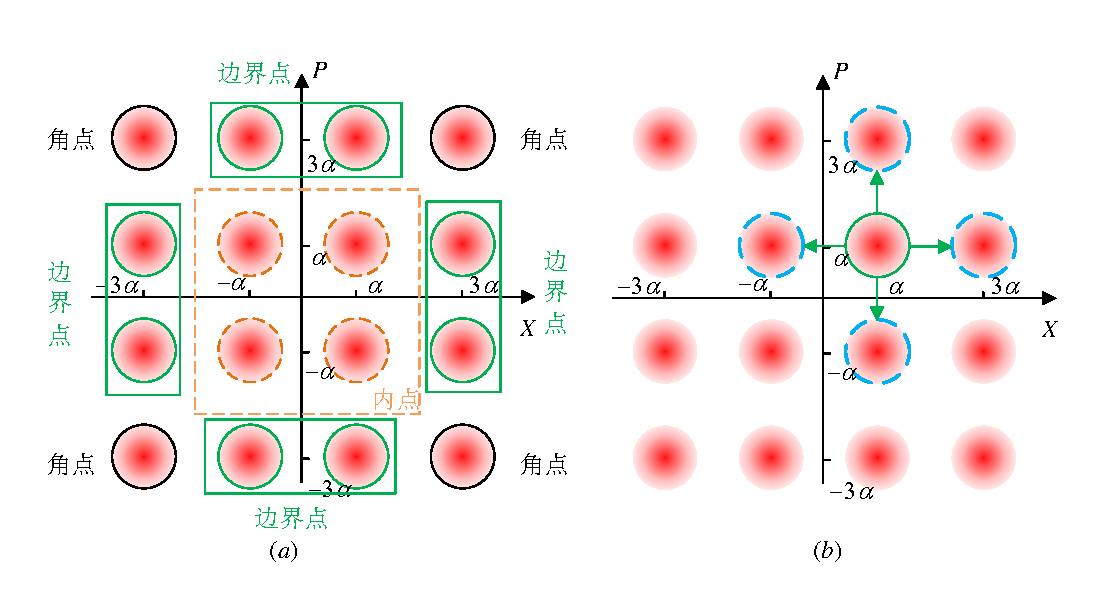
\includegraphics[width=0.8\textwidth]{figures/chap3/QAM-nearbor}
  \caption{QAM信号三类点和最近邻点示意图}
  \label{fig:QAM-nearbor}
\end{figure}

因为
\begin{equation}
\begin{split}
(\hat{Z}^2)_{ii} &= \sum_k Z_{ik}Z_{ki}    \\
                 &=\sum_{k \neq i} \exp\{- |\alpha|^2 [(u_i-u_k)^2 + (v_i-v_k)^2]\}.
\end{split}
\end{equation}
如果忽略高阶小量,那么只有最近邻点的值保留下来,所以
\begin{equation}
(\hat{Z}^2)_{ii} \approx \begin{cases}
                            2 e^{- 4|\alpha|^2} & \text{角点} \\
                            3 e^{- 4|\alpha|^2} & \text{边界点} \\
                            4 e^{- 4|\alpha|^2} & \text{内点} .
                         \end{cases}
\end{equation}
所以由\ref{eq:SRM-Pe}式,QAM信号的平方根检测渐近错误概率为
\begin{equation}
\begin{split}
P_e & \approx 1 - \frac{1}{M}\sum_{i=1}^M |1 - \frac{1}{8} (\hat{Z}^2)_{ii}|^2 \\
   & \approx 1 - \frac{1}{M}\sum_{i=1}^M (1 - \frac{1}{4} (\hat{Z}^2)_{ii}) \\
   & \approx  \frac{1}{4M} [4\times 2e^{- 4|\alpha|^2} + 4(L-2) \times 3e^{- 4|\alpha|^2} \\
   & \qquad  + (L-2)^2 \times 4e^{- 4|\alpha|^2}] \\
   & =      (1 - \frac{1}{L})  e^{- 4|\alpha|^2}. 
\label{eq:QAM-SRM-approx}   
\end{split}
\end{equation}
因为平方根检测在平均光子数较大的时候,与最优检测几乎一致,所以可以认为
该渐近性能就是Helstrom极限在平均光子数较大时的渐近性能。
比较\ref{eq:QAM-SQL-approx}式和\ref{eq:QAM-SRM-approx}式可知,
采用量子检测的手段,接收机的性能将有指数倍的增益。

\section{QAM信号Bondurant接收机}
为了探测QAM信号,我们借鉴了QPSK信号第一种Bondurant接收机的思想,
将这种接收策略应用到QAM信号的接收。
如图\ref{fig:QAM-Bondurant-receiver}所示,这种接收机由一个高透过率的波束分束器、
一个单光子探测器和一个与信号场高相干的本振构成。

\begin{figure}
\centering
  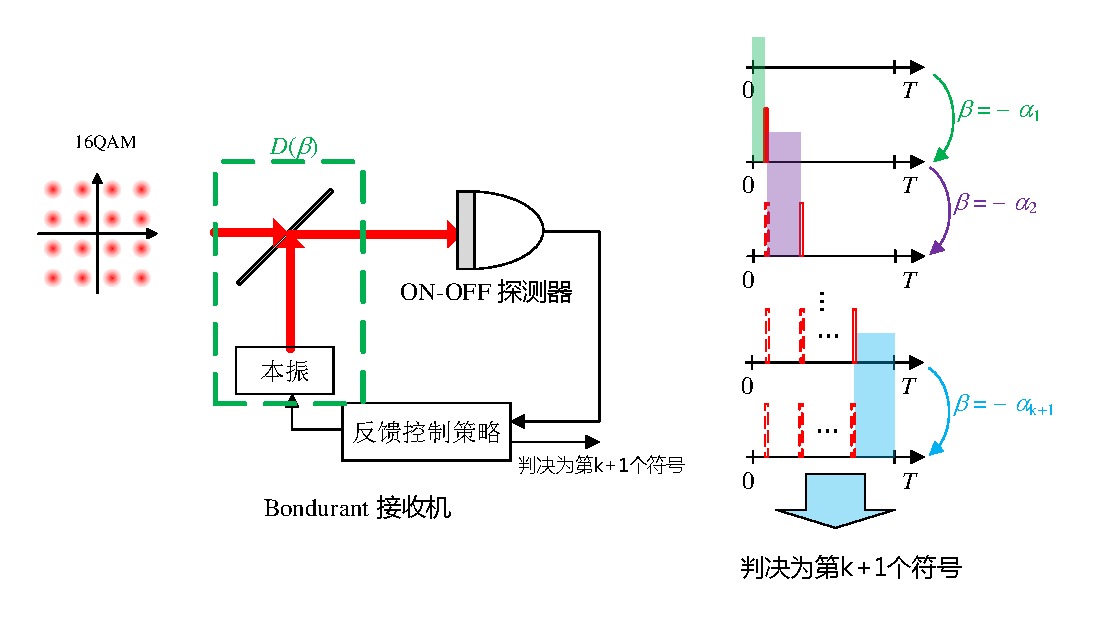
\includegraphics[width=\textwidth]{figures/chap3/Bondurant-receiver}
  \caption{QAM信号Bondurant接收机和反馈策略示意图}
  \label{fig:QAM-Bondurant-receiver}
\end{figure}

为了说明接收机接收过程,我们将$M$阶QAM信号按顺序编号为$\alpha_1,\alpha_2,...,\alpha_M$。
记符号到来的初始时刻为$t=0$,符号持续的时间为$T$。
接收机按照图\ref{fig:QAM-Bondurant-receiver}所示的策略
进行反馈控制,反馈策略可以归纳如下:

1.在$t=0$时刻,控制本振使得位移操作$\hat{D}(\beta) = \hat{D}(-\alpha_1)$,
  即将符号1归零,同时选择假设$H_1$:当前的符号为$\alpha_1$。
  
2.在任意$0<t<T$时刻,如果没有发生光子计数事件,
  那么保持当前的假设和本振,继续接收信号;
  如果在$t_i$时刻发生了第$i$个光子计数事件,
  那么将当前的假设由$H_i$转变为$H_{i+1}$,
  同时控制本振归零下一个符号,即$\hat{D}(\beta) = \hat{D}(-\alpha_{i+1})$。
  然后继续接收信号。
  
3.重复步奏2直到$t=T$时刻,信号接收完毕,
  输出当前的假设$H_i$作为对该符号的判决。
  
假设发送的信号是$\alpha_k$,
在该符号周期内,发生了$k'$个光子计数事件,
这$k'$个光子计数事件发生的时间为$t_i,(i=1,2,...,k')$,
仅当$k' = k-1$的时候,接收机判决输出的假设为$H_k$,
它对应的概率分布为
\begin{equation}
p(t_1,t_2,...,t_{k-1}|k) = \prod_{i=1}^{k-1} w(t_i|k).
\end{equation}
假定$t_0=0$,这里
\begin{equation}
w(t_i|k) =  \frac{|\alpha_k - \alpha_i|^2}{T} \exp(-|\alpha_k - \alpha_i|^2 \frac{t_i-t_{i-1}}{T}) .
\label{eq:w-cond}
\end{equation}
代表在发送的信号为$\alpha_k$时,
在半开时间区间$(t_{i-1}, t_i]$内,
恰好在$t_i$时刻发生了光子计数
的概率密度。
所以,在发送的信号为$\alpha_k$时接收机判决为$\alpha_k$的
条件概率为
\begin{equation}
\Pr{k|k} = \int\int\cdots\int_{0<t_1<t_2<\cdots<t_{k-1}<T} p(t_1,t_2,...,t_{k-1}|k) dt_1 dt_2 \cdots dt_{k-1}.
\label{eq:QAM-cond-prob}
\end{equation}

对于第$k$个信号,上述积分为$k-1$重,
为了便于分析,对给定的符号$\ket{\alpha_k}$定义如下函数
\begin{equation}
Q_i^k(t) = \begin{cases}
            1 & i=1, \\
            \int_t^1  dt_{i-1}' n_{k,i-1} e^{-n_{k,i-1}(1-t)} Q_{i-1}(t_{i-1}') & 1 < i \le k.
         \end{cases}
\label{eq:Q-func}
\end{equation}
上式中$n_{k,l} = |\alpha_k - \alpha_l|^2$。
接下来,我们利用\ref{eq:w-cond}式将\ref{eq:QAM-cond-prob}式进行改写,
作变量代换$t_i \rightarrow T t_{k-i}'$,那么\ref{eq:QAM-cond-prob}式化为
\begin{equation}
\begin{split}
\Pr{k|k} = & \int_{0}^1 dt_{k-1}' n_{k,1} e^{-n_{k,1} t_{k-1}'}          \int_{t_{k-1}'}^1 dt_{k-2}'   \frac{n_{k,2}}{T} e^{-n_{k,2} (t_{k-2}'-t_{k-1}')} \\
           & \cdots    \int_{t_1'}^1 dt_1' n_{k,k-1} e^{-n_{k,k-1} (t_1'-t_2')}.
\end{split}
\end{equation}

对式\ref{eq:Q-func}反复递归可得$Q_k(t)$表达式,对照上式有$\Pr{k|k} = Q_k(0)$。
因此,我们可以用递归式\ref{eq:Q-func}来求上述积分。

下面,我们来证明一个断言,对给定的$k,m$和从充分大的$\alpha$,
存在一组与$t$无关的,关于$n_0 = |\alpha|^2$的$m-1$阶多项式$A_i^m \ge 0$,
使得下式成立
\begin{equation}
\begin{split}
Q_m^k(t) \ge 1 - \sum_{i=1}^{m-1} A_i^m e^{-n_{k,i}(1-t)}, (m=1,2,...,k).
\end{split}
\label{eq:Q-expand}
\end{equation}
当$m=1$时,显然成立。假设上式在$m<1$时成立,那么在$m+1$时,有
\begin{equation}
\begin{split}
Q_{m+1}^k(t) &\ge \int_t^1  dt_{m}' n_{k,m} e^{-n_{k,m}(1-t)} (1 - \sum_{i=1}^{m-1} A_i^m e^{-n_{k,i}(1-t_m)} ) \\
             &\ge 1 - \left( \sum_{\substack{1\le i \le m-1 \\
                n_{k,i} = n_{k,m}} }  n_{k,m}A_i^{m} -1\right) e^{-n_{k,m}(1-t)}  \\
             & \quad - \sum_{\substack{1\le i \le m-1 \\
                n_{k,i} \neq n_{k,m}}} \left(-\frac{n_{k,m}}{n_{k,i} - n_{k,m}} A_i^m e^{-n_{k,i}(1-t)}  + \frac{n_{k,m}}{n_{k,i} - n_{k,m}} A_i^m e^{-n_{k,m}(1-t)}    \right) .
\end{split}
\label{eq:Q-ineq}
\end{equation}
因此,只要取正$m+1$阶多项式使得
\begin{equation}
\begin{split}
A_i^{m+1} &\ge -\frac{n_{k,m}}{n_{k,i} - n_{k,m}} A_i^m , i<m \text{且} n_{k,i} \neq n_{k,m}\\
A_i^{m+1} &\ge 0 , i<m \text{且} n_{k,i} = n_{k,m}\\
A_m^{m+1} &\ge -1 + \sum_{\substack{1\le i \le m-1 \\
                n_{k,i} = n_{k,m}} }  n_{k,m}A_i^{m} + \sum_{\substack{1\le i \le m-1 \\
                n_{k,i} \neq n_{k,m}}} \frac{n_{k,m}}{n_{k,i} - n_{k,m}} A_i^m .
\end{split}
\end{equation}
成立即可,于是命题得证。
利用这个命题,因为$n_{k,i} \ge 4|\alpha|^2,(k \neq i)$,
所以QAM信号Bondurant接收机的渐近性能上界为
\begin{equation}
P_e \le C_{M-1}(|\alpha|^2) e^{-4|\alpha|^2}.
\label{eq:QAM-Bondurant-approx-err}
\end{equation}
其中$C_{M-1}(|\alpha|^2)$是$|\alpha|^2$的$M-1$阶正多项式。
作为一个特例,如果$n_{k,i} \neq n_{k,m}$对所有的$i\neq m$成立,
那么式\ref{eq:Q-ineq}中的第一个求和不存在,
从而可以将命题加强为:
存在一组与$t$和$\alpha$无关的常数$A_i^m \ge 0$,使得\ref{eq:Q-expand}式成立。
从而存在足够大的常数$C$使得当$|\alpha| \gg 1$时有
\begin{equation}
P_e \le C e^{-4|\alpha|^2}.
\label{eq:QAM-Bondurant-approx-err-2}
\end{equation}
这与最优量子检测的渐进平均错误概率
只相差一个常系数。


另一方面,对于充分大的$\alpha$,有
\begin{equation}
w(t_i|k) \ge \frac{4|\alpha|^2}{T} \exp(-4|\alpha|^2 \frac{t_i-t_{i-1}}{T}) .
\end{equation}
所以
\begin{equation}
\begin{split}
\Pr{k|k} \ge & \int_{0}^1 dt_{k-1}' 4|\alpha|^2 e^{-4|\alpha|^2 t_{k-1}'}    \int_{t_{k-1}'}^1 dt_{k-2}'   4|\alpha|^2 e^{-4|\alpha|^2 (t_{k-2}'-t_{k-1}')} \\
           & \cdots    \int_{t_1'}^1 dt_1' 4|\alpha|^2 e^{-4|\alpha|^2 (t_1'-t_2')} \\
         = & 1- \left[ 4|\alpha|^2 + (4|\alpha|^2)^2 + \cdots + (4|\alpha|^2)^{k-2} \right] e^{-4|\alpha|^2}  \\
         = & 1 - \frac{(4|\alpha|^2)^{k-1}-4|\alpha|^2}{4|\alpha|^2-1} e^{-4|\alpha|^2}.
\end{split}
\end{equation}
因此,也可以得到渐近误差上界为式\ref{eq:QAM-Bondurant-approx-err}。
对比式\ref{eq:QAM-SQL-approx}和\ref{eq:QAM-Bondurant-approx-err},
可知QAM信号Bondurant接收机比外差接收具有指数倍增益,它的渐近性能
与量子最优检测性能只相差一个多项式。


为了精确求解接收机的平均错误概率,需要计算多重积分\ref{eq:QAM-cond-prob},
对于低维情况如16-QAM信号,还能在比较快的时间里计算出来,
但是对于更高维情况如36-QAM、64-QAM信号,
计算时间较慢。这里采用Monte Carlo仿真的方法计算接收机的性能,
仿真步奏可以归纳如下:

1. 从信号的初始时刻$t=0$开始,选择假设$H_1$,
   并控制本振使得$\beta=-\alpha_1$。
   
2. 设当前$t$时刻发生的光子计数个数为$i$,
   由于光子到达的过程可以看做一个泊松点过程,
   因此两个光子到达的时间间隔服从强度为$I$的指数分布\cite{hs2009sjgc}。
   这里$I=|\alpha_m-\alpha_{i+1}|/T$是当前进入探测器的光强,
   $\alpha_m$是实际的信号,$\beta = -\alpha_{i+1}$。
   因此可以通过服从该指数分布的随机数发生器产生一个随机数$\tau$作为
   下一个光子发生前所经历的时间。

3. 如果$t+\tau<T$,那么将当前时刻更新为$t + \tau$,
   更新当前的假设为$H_{i+1}$,并利用反馈控制本振使得$\beta = -\alpha_{i+2}$,
   即归零符号$i+2$,然后继续重复步骤1;
   如果$t+\tau \ge T$,那么说明在信号剩下的时间
   里面没有光子计数事件发生,输出当前的假设作为判决输出,
   判断接收机是否判断错误。
   
4. 重复步奏2~3足够多次,记录接收机判断错误的频率作为接收机平均错误
   概率的估计值。
   
这种方法的计算精度与问题的维度无关\cite{mcbook},
计算时间只随仿真点数和信号数目线性增长,
能够有效求解高阶QAM接收机平均错误概率的问题。
每一次仿真都是一个独立重复事件,用随机变量$\xi$
表示输出结果,$\xi=0$表示接收机判断错误,
$\xi=1$表示接收机判断正确。那么有
\begin{equation}
\E \xi = p, \Var \xi = p(1-p).
\end{equation}
重复该独立事件$N$次,得到估计值
\begin{equation}
\tilde{p} = \frac{1}{N} \sum_{i=1}^N \xi_i.
\end{equation}
该统计量的期望与方差为
\begin{equation}
\E \tilde{p} = p, \Var \tilde{p} = \frac{p(1-p)}{N}.
\end{equation}
若$p \ll 1$,那么它的标准差约为$\sqrt{p/N}$,
为了得到一定精度的仿真结果,可以选取适当的$N$
和一个小量$\epsilon$,使得$\Delta p / p < \epsilon$。
当$N$很大时,随机变量$\tilde{p}$可以认为近似服从正态分布,
可以利用$3\sigma$原则选取$\Delta p = 3 \sqrt{\Var \tilde{p}}$
因此若取$\epsilon=0.1$计算精度,那么有
\begin{equation}
N > \frac{300}{p}.
\end{equation}
例如,要在平均错误概率大约在$10^{-5}$的时候,
保证$\epsilon=0.1$的计算精度,需要的仿真点个数为$3\times10^7$。

\begin{figure}
\centering
  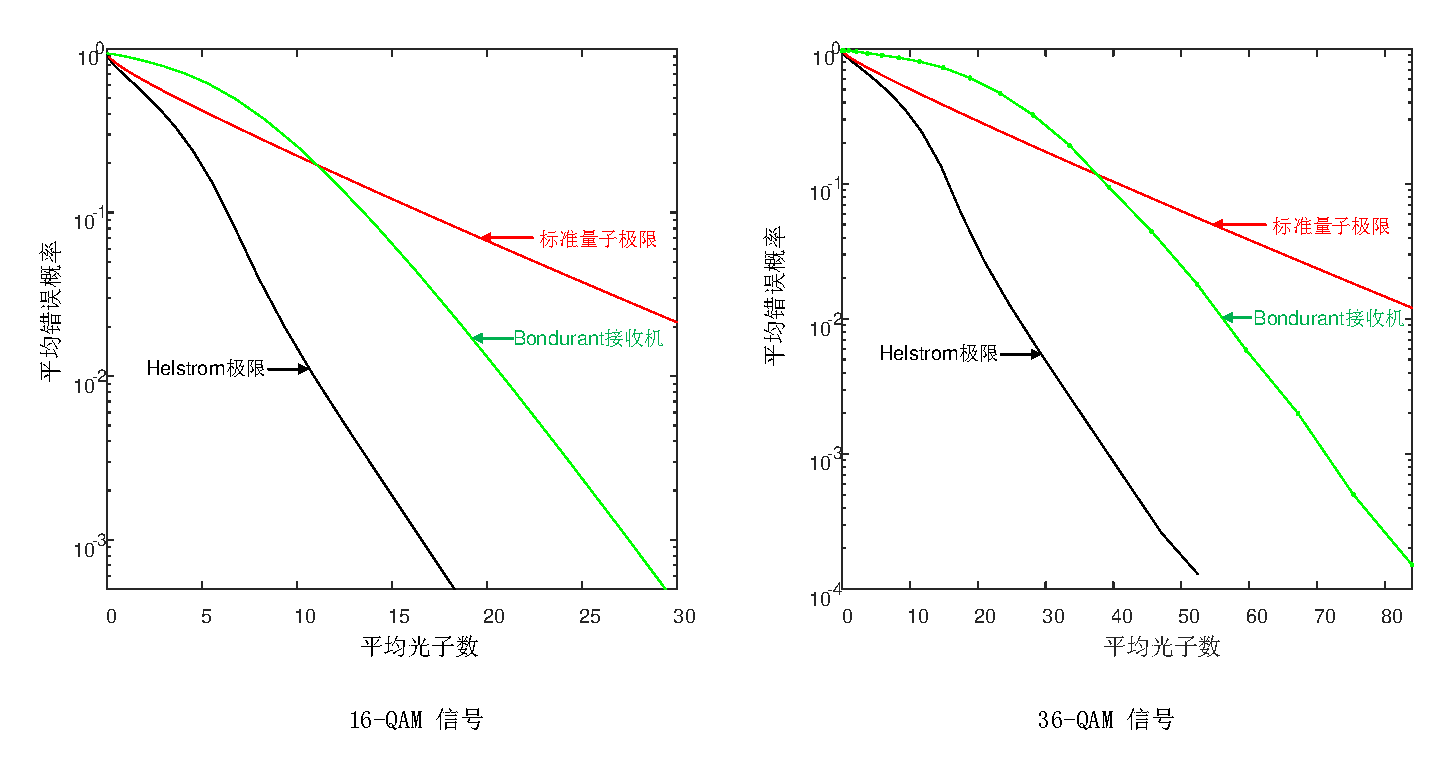
\includegraphics[width=\textwidth]{figures/chap3/QAM-bondurant-error}
  \caption{QAM信号Bondurant接收机性能曲线}
  \label{fig:QAM-bondurant-error}
\end{figure}


我们以16-QAM信号和36-QAM信号位移,
通过数值仿真分析,得到Bondurant接收机的性能曲线如图\ref{fig:QAM-bondurant-error}
所示。从图中可以看到,当平均光子数较小的时候,
Bondurant接收机性能没有突破标准量子极限,
当平均光子数较大时,Bondurant接收机的性能
就可以突破标准量子极限,并且随着光子数的增大,
这种优势就越大,这与上面的理论分析一致。




\section{QAM信号自适应分区检测接收机}

由于Bondurant接收机需要实时反馈控制,
对系统反馈带宽和资源消耗要求较高,
不利于工程实现。因此,可以借鉴用自适应分区检测的方法加以改进。
我们将QPSK信号的自适应分区检测接收机推广到任意QAM信号,
研究在QAM信号配置下,这种接收机的性能是否也能突破标准量子极限。

\begin{figure}
\centering
  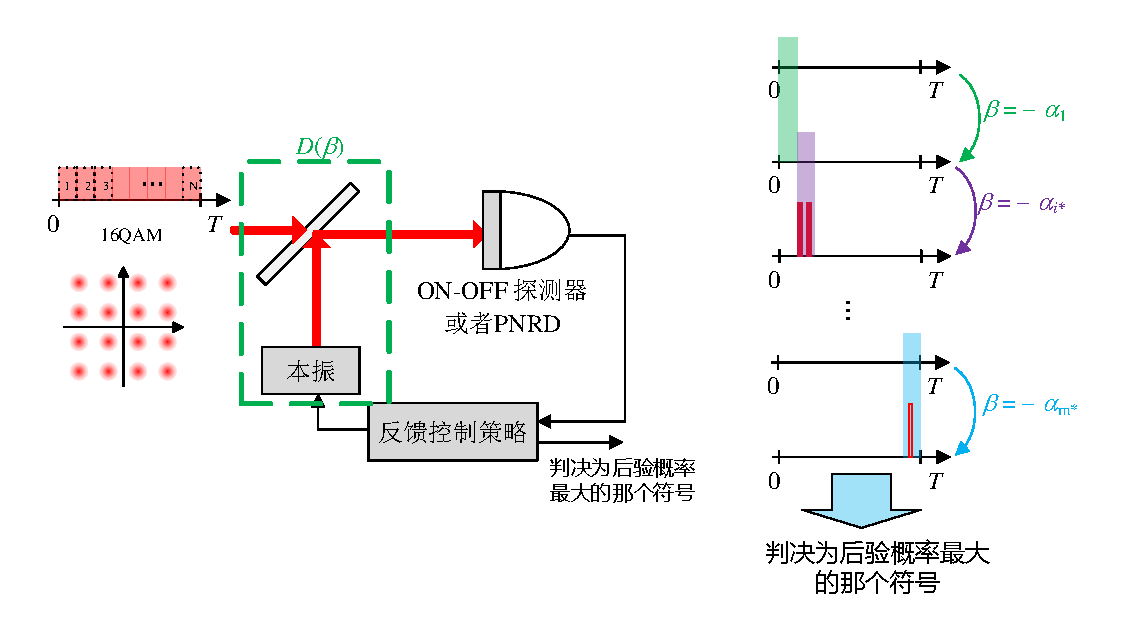
\includegraphics[width=\textwidth]{figures/chap3/QAM-ADP-receiver}
  \caption{QAM信号自适应分区检测接收机和反馈控制策略示意图}
  \label{fig:QAM-ADP-receiver}
\end{figure}

如图\ref{fig:QAM-ADP-receiver}所示,
QAM信号自适应分区检测接收机结构与Bondurant接收机一致,
所不同的在接收策略上。
接收机将信号在时间上分成若干个分区,在每一个分区里面,
不论是否有光子计数事件发生,本振都是恒定的。
只有分区结束了,才会采用反馈控制策略去更新本振,
因此对反馈带宽的要求大大降低了。


在信号的起始时刻,将每个符号的先验概率设为相同$P_m^{prior} = 1/M$。
并随机选择一个符号进行归零,即控制本振使得$\hat{D}(\beta)=\hat{D}(-\alpha_{i_0})$。
设总分区数目为$N$,
在第$i$个分区时,先验概率为$P_{m,i}^{prior}$,
控制参数$\beta = -\alpha_{u_i},(u_i \in \{1,2,..,M\})$。
设第$i$个分区结束了之后,对于ON-OFF探测器,
探测器则只能判断是否有光子计数发生,对应的条件概率为
\begin{equation}
P\{k|\alpha_m, \beta\} = \begin{cases}
                        1 - e^{-|\alpha_m - \beta|^2/N}, & k>0, \text{ON}\\
                        e^{-|\alpha_m - \beta|^2/N},     & k=0, \text{OFF}.
                       \end{cases}
\end{equation}
如果是具有光子数分辨能力的探测器(PNRD),则对应的条件概率为
\begin{equation}
P\{k|\alpha_m, \beta\} = e^{-|\alpha_m - \beta|^2/N} \frac{|\alpha_m - \beta|^{2k}}{N k!}.
\label{eq:QAM-ADP-cond-prob}
\end{equation}
那么在第$i$个分区结束的时候,对应的后验概率为
\begin{equation}
P_{m,i}^{post} = \frac{P_{m,i}^{prior} P\{k|\alpha_m, \beta=-\alpha_{u_i}\}}{\sum_{m=1}^M P_{m,i}^{prior} P\{k|\alpha_m, \beta=-\alpha_{u_i}\}}.
\label{eq:QAM-ADP-post-prob}
\end{equation}
其中后验概率最大的符号为
\begin{equation}
m^* = \arg\max_m P_{m,i}^{post}.
\end{equation}
若所有的分区都已经探测完毕,则输出假设$H_{m^*}$。
否则将下一个分区的先验概率设为$P_{m,i+1}^{prior} = P_{m,i}^{post}$,
同时通过反馈控制本振使得$\beta = -\alpha_{m^*}$,
即归零后验概率最大的符号,选择当前的假设为$H_{m^*}$。
然后重复上述步骤直到所有的分区都探测完毕。

% 对于任意符号$\alpha_k$,我们来计算条件概率$\Pr{k|k}$,
% 即输出结果也为$\alpha_k$的概率。
% 在这种情况下,不妨假定$N$个分区中最后发生光子计数
% 的区间是第$K-1$个,那么最后$K$个分区的
% 位移参数$\beta = -\alpha_k$,且这$K$个分区
% 没有发生光子计数事件的概率为1。
% 而在前$N-K$个分区里面,发生光子计数的分区数目不超过$M-1$,
% 设$N$个分区发生光子计数数目分别为$o_i$,
% 对应的控制参数分别为$\beta_i$。
% 定义集合
% \begin{equation}
% \Omega_k = \{o_1,o_2,...,o_N,\beta_1,\beta_2,...,\beta_N \}$
% \end{equation}
% 那么
% \begin{equation}
% \Pr{k|k} = \sum_{K=0}^{M} \sum_{o_1,o_2,...,o_N} \sum_{\beta_1,\beta_2,...,\beta_{K-1},\beta_{K}=-\alpha_k,...,\beta_{M}=-\alpha_k} P\{K, o_1,o_2,..,o_N,\beta_1,\beta_2,...,\beta_N | \alpha_k\}
% \end{equation}



可以预计随着分区数目增大,接收机的性能会越来越好,
当$N\rightarrow\infty$时,就与Bondurant接收机的实时
反馈控制一致了。
在这种极限下,如果一个分区没有光子计数事件发生,
那么条件概率
\begin{equation}
P\{k=0|\alpha_m, \beta=\alpha_{u_i}\} = e^{-|\alpha_m - \alpha_{u_i}|^2/N} \frac{1}{N}.
\end{equation}
中最大的仍然是$\alpha_{u_i}$,即最大的仍然是当前选择的符号。
因此接收机只在有光子计数事件发生的时候,才更改本振。
所以在$N\rightarrow\infty$的极限情况,
只需要修改Bondurant接收机的第3步即可。
蒙特卡洛仿真步奏可以归纳如下:

1. 从信号的初始时刻$t=0$开始,选择假设$H_1$,
   并控制本振使得$\beta=-\alpha_1$,
   此时$M$个先验概率为$P_{m,1}^{prior} = 1/M,(m=1,2,...,M)$。

2. 设当前$t$时刻发生的光子计数个数为$i-1$,
   当前位移参数$\beta = \alpha_{u_i}$,
   由于光子到达的过程可以看做一个泊松点过程,
   所以距下一个光子计数事件发生的时间间隔服从强度为$I_{m,u_i}$的指数分布\cite{hs2009sjgc}。
   这里$I_{m,u_i}=|\alpha_m-\alpha_{u_i}|/T$是当前进入探测器的光强,
   $\alpha_m$是实际的信号,$\beta = -\alpha_{u_i}$是当前的控制参数。
   因此可以通过服从该指数分布的随机数发生器产生一个随机数$\tau$作为
   下一个光子发生前所经历的时间。

3. 如果$t+\tau<T$,那么将当前时刻更新为$t + \tau$,
   该事件对应的条件概率为
   \begin{equation}
    P\{\Delta t = \tau|\alpha_m, \beta=\alpha_{u_i}\} = e^{-I_{m ,u_i}\tau/T} \frac{I_{m ,u_i}}{T}.
    \label{eq:QAM-ADP-cond-prob-2}
   \end{equation}
   根据上式和\ref{eq:QAM-ADP-post-prob}可以计算出该事件发生后$M$个后验概率
   $P_{m,i}^{post}$,从从选择出最大后验概率对应的符号$\alpha_{u_{i+1}}$,
   然后更新当前的假设为$H_{u_{i+1}}$,并利用反馈控制本振使得$\beta = -\alpha_{u_{i+1}}$,
   即归零符号$u_{i+1}$,然后继续重复步骤1;
   如果$t+\tau \ge T$,那么说明在信号剩下的时间
   里面没有光子计数事件发生,输出当前的假设作为判决输出,
   判断接收机是否判断错误。
   
4. 重复步奏2~3足够多次,记录接收机判断错误的频率作为接收机平均错误
   概率的估计值。
   

\begin{figure}
\centering
  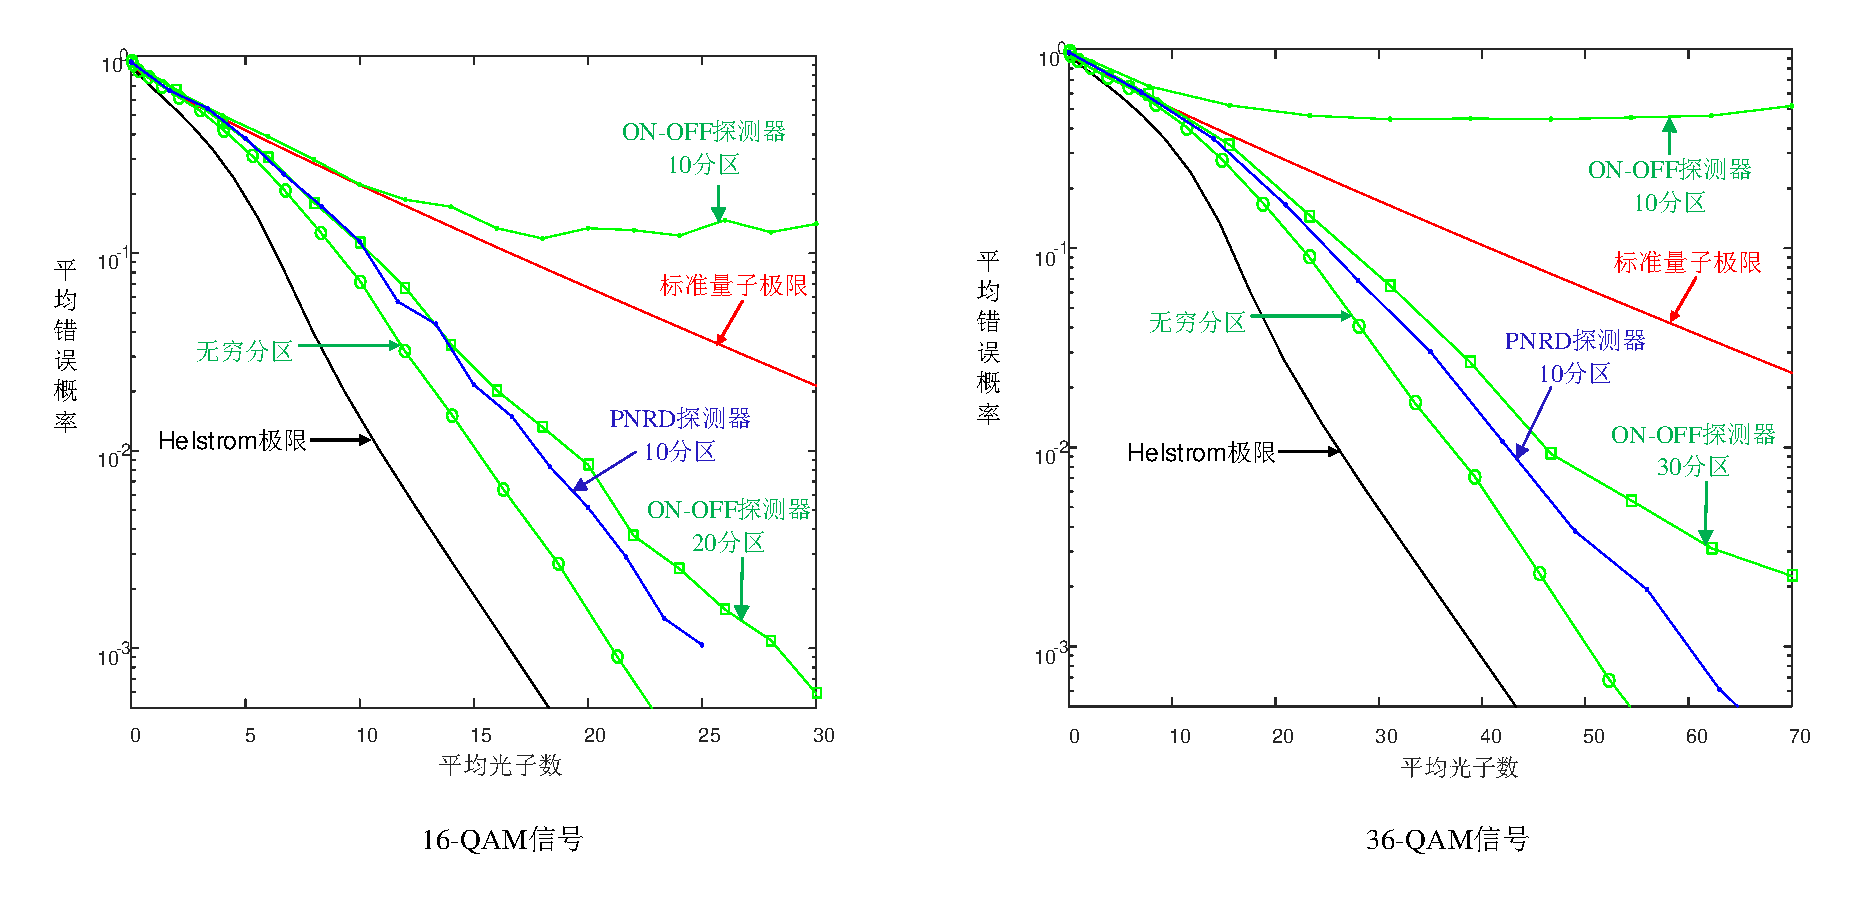
\includegraphics[width=\textwidth]{figures/chap3/QAM-ADP-error}
  \caption{QAM信号自适应分区检测接收机性能曲线}
  \label{fig:QAM-ADP-error}
\end{figure}
 
 
我们选取了16-QAM和36-QAM信号进行仿真分析,
并且针对不同分区数目和不同的探测器进行了研究。
Monte Carlo仿真结果如图\ref{fig:QAM-ADP-error}所示。
对比ON-OFF探测器不同分区的曲线,
可以看出随着分区数目的增大,
接收机的平均错误概率都在降低,
当分区数目趋近于无穷时,
错误概率达到最低,从图中可以看到,
它可以在任意光子数都能突破标准量子极限。
但是分区数目较少的时候,比如只有10各分区,
可以看到16-QAM信号和36-QAM信号的
自适应分区检测接收机都没能突破标准量子极限。
并且随着光子数增加,接收机性能出现了饱和现象。
而这种现象可以通过具有光子数分辨能力的探测器
解决。对比都采用10个分区的情况下,
ON-OFF探测器和PNRD探测器,
采用PNRD探测器都能够突破标准量子极限,
没有出现饱和的现象,这是因为每一个分区
发生的光子计数数目也携带信息,
当光子数较强的时候,每个分区发生多个光子
计数时间的概率大大增加,而这些信息
采用ON-OFF探测器是无法获取的。
从图中还可以看到,对于16-QAM信号,
10分区的PNRD和20分区的ON-OFF的性能接近,
对于36-QAM信号,
10分区的PNRD和30分区的ON-OFF的性能接近,
因此PNRD可以在达到相同的错误概率的情况下
减少分区数目。此外,采用PNRD能够有效地
克服暗计数、模式适配等非理想因素也被报道\cite{izumi2013quantum, li2013suppressing}。
通过仿真分析,我们可以认为对于一般的QAM信号,
这种接收机都能突破标准量子极限。
在工程实现的时候,可以通过PNRD增加系统鲁棒性
减少分区数目,从而减少反馈带宽。






\section{QAM信号混合接收机}
另外一种实现多元调制量子接收机的方法是利用
一个混合接收方案\cite{muller2012quadrature,李科2014}。
对于一般的QAM信号,混合接收机该如何设计
是这一节的主要内容。

\begin{figure}
\centering
  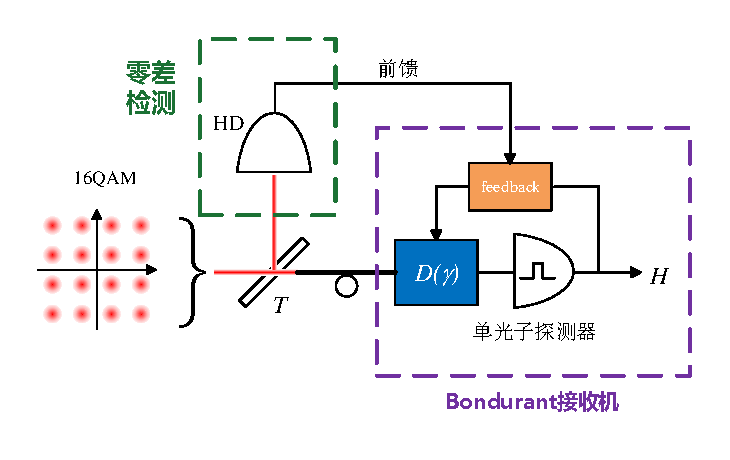
\includegraphics[width=0.7\textwidth]{figures/chap3/QAM-Hybrid-receiver}
  \caption{QAM信号混合接收机示意图}
  \label{fig:QAM-Hybrid-receiver}
\end{figure}

对于QAM信号,混合接收机可以用如图\ref{fig:QAM-Hybrid-receiver}所示的
结构实现。它包含两个部分——零差接收和Bondurant接收机。
M阶QAM信号首先经过一个透过率为$T$的分束器(BS)分成两部分,一部分给零差接收机(HD),
零差接收机通过一组POVM测量进行探测,
\begin{equation}
\hat{\Pi}_v^{HD} = \int_{D_v} dp \ket{p}\bra{p}, v\in \Omega.
\end{equation}
其中符号$\Omega$与式\ref{eq:QAM-omega}定义一致,
积分区域定义如下
\begin{equation}
\begin{split}
D_v = \{p| D_L(v)r\alpha < p \le D_U(v) r\alpha\}.
\end{split}
\end{equation}
其中$r=\sqrt{1-T}$是反射系数,$D_L$和$D_U$是式\ref{eq:LU-fun}
定义的两个上下界函数。
如图\ref{fig:Q-Bondurant-displacemet}所示,
零差检测不同的判定区域对应一个按照P分量分割的分区,
经过零差接收后,就可以知道信号所在的区域。


\begin{figure}
\centering
  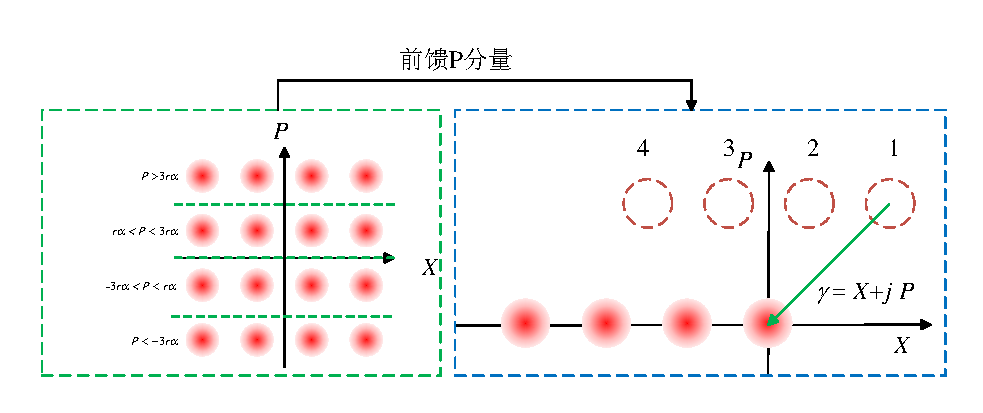
\includegraphics[width=\textwidth]{figures/chap3/Q-Bondurant-displacemet}
  \caption{四态区分的Bondurant接收机位移操作示意图}
  \label{fig:Q-Bondurant-displacemet}
\end{figure}

正确探测出信号所在区域的概率可以用下式计算出来
\begin{equation}
\begin{split}
P^{HD}\{v|\alpha_{uv}\} &= \int_{D_v}|\bra{p}\ket{r\alpha_{uv}}|^2 dp  \\
   &= \frac{1}{2} \left( \erf(\sqrt{2} (D_U(v)-v) r\alpha) -  \erf(\sqrt{2} (D_L(v)-v) r\alpha) \right).
\end{split}
\end{equation}
代入上下界得到
\begin{equation}
\begin{split}
P^{HD}\{v|\alpha_{uv}\} = \begin{cases}
                            \frac{1}{2}\left( 1 + \erf(\sqrt{2}r\alpha) \right)  & v \neq \pm (L-1), \\
                            \erf(\sqrt{2}r\alpha) & v = \pm (L-1).
                          \end{cases}
\end{split}
\end{equation}
所以该零差接收机的平均正确概率为
\begin{equation}
P_c^{HD} = \frac{1}{L}\left(1 + (L-1)\erf(\sqrt{2}r\alpha) \right)
\end{equation}
当光子数很大时,利用余误差函数的Chernoff界\cite{chang2011chernoff}可得
\begin{equation}
\begin{split}
P_c^{HD} \approx 1 - (1-\frac{1}{L}) e^{-2r^2\alpha^2}.
\end{split}
\label{eq:QAM-Hybrid-approx-1}
\end{equation}
若采用50:50的分束器,那么
\begin{equation}
P_c^{HD} \approx 1 - (1-\frac{1}{L}) e^{-\alpha^2}.
\end{equation}


零差接收机探测的结果将前馈给后面的位移接收机,
用于位移接收机调整位移操作的策略控制。
如图\ref{fig:Q-Bondurant-displacemet} 所示,
如果零差探测得到正确的结果,那么后面就变成一个
$L$态区分问题,这个$L$态区分可以用Boundrant接收机实现。
为了进行位移操作,Bondurant接收需要知道
位移参数$\gamma = X + jP$的$P$分量,
对于不同的分区,这个分量值不同,
对于该$L$态区分问题,这个分量的值是相同的,
这个值通过前面的零差接收机前馈得到。



Bondurant接收机的接收策略如图\ref{fig:Q-Bondurant-displacemet-strategy}  所示,
在信号到达Boundrant接收机时,
Bondurant接收机利用前馈得到的$P$值,
开始调整本振归零符号1,
接着在每一个光子计数时间发生的时候,
按照$1\rightarrow 2 \rightarrow ... \rightarrow L$顺序
依次归零对应符号。
理想情况下,对于图中信号3,由于最多发生
2个光子计数事件,图\ref{fig:Q-Bondurant-displacemet-strategy} (\textit{a}.4)
的情况是不能到达的。

\begin{figure}
\centering
  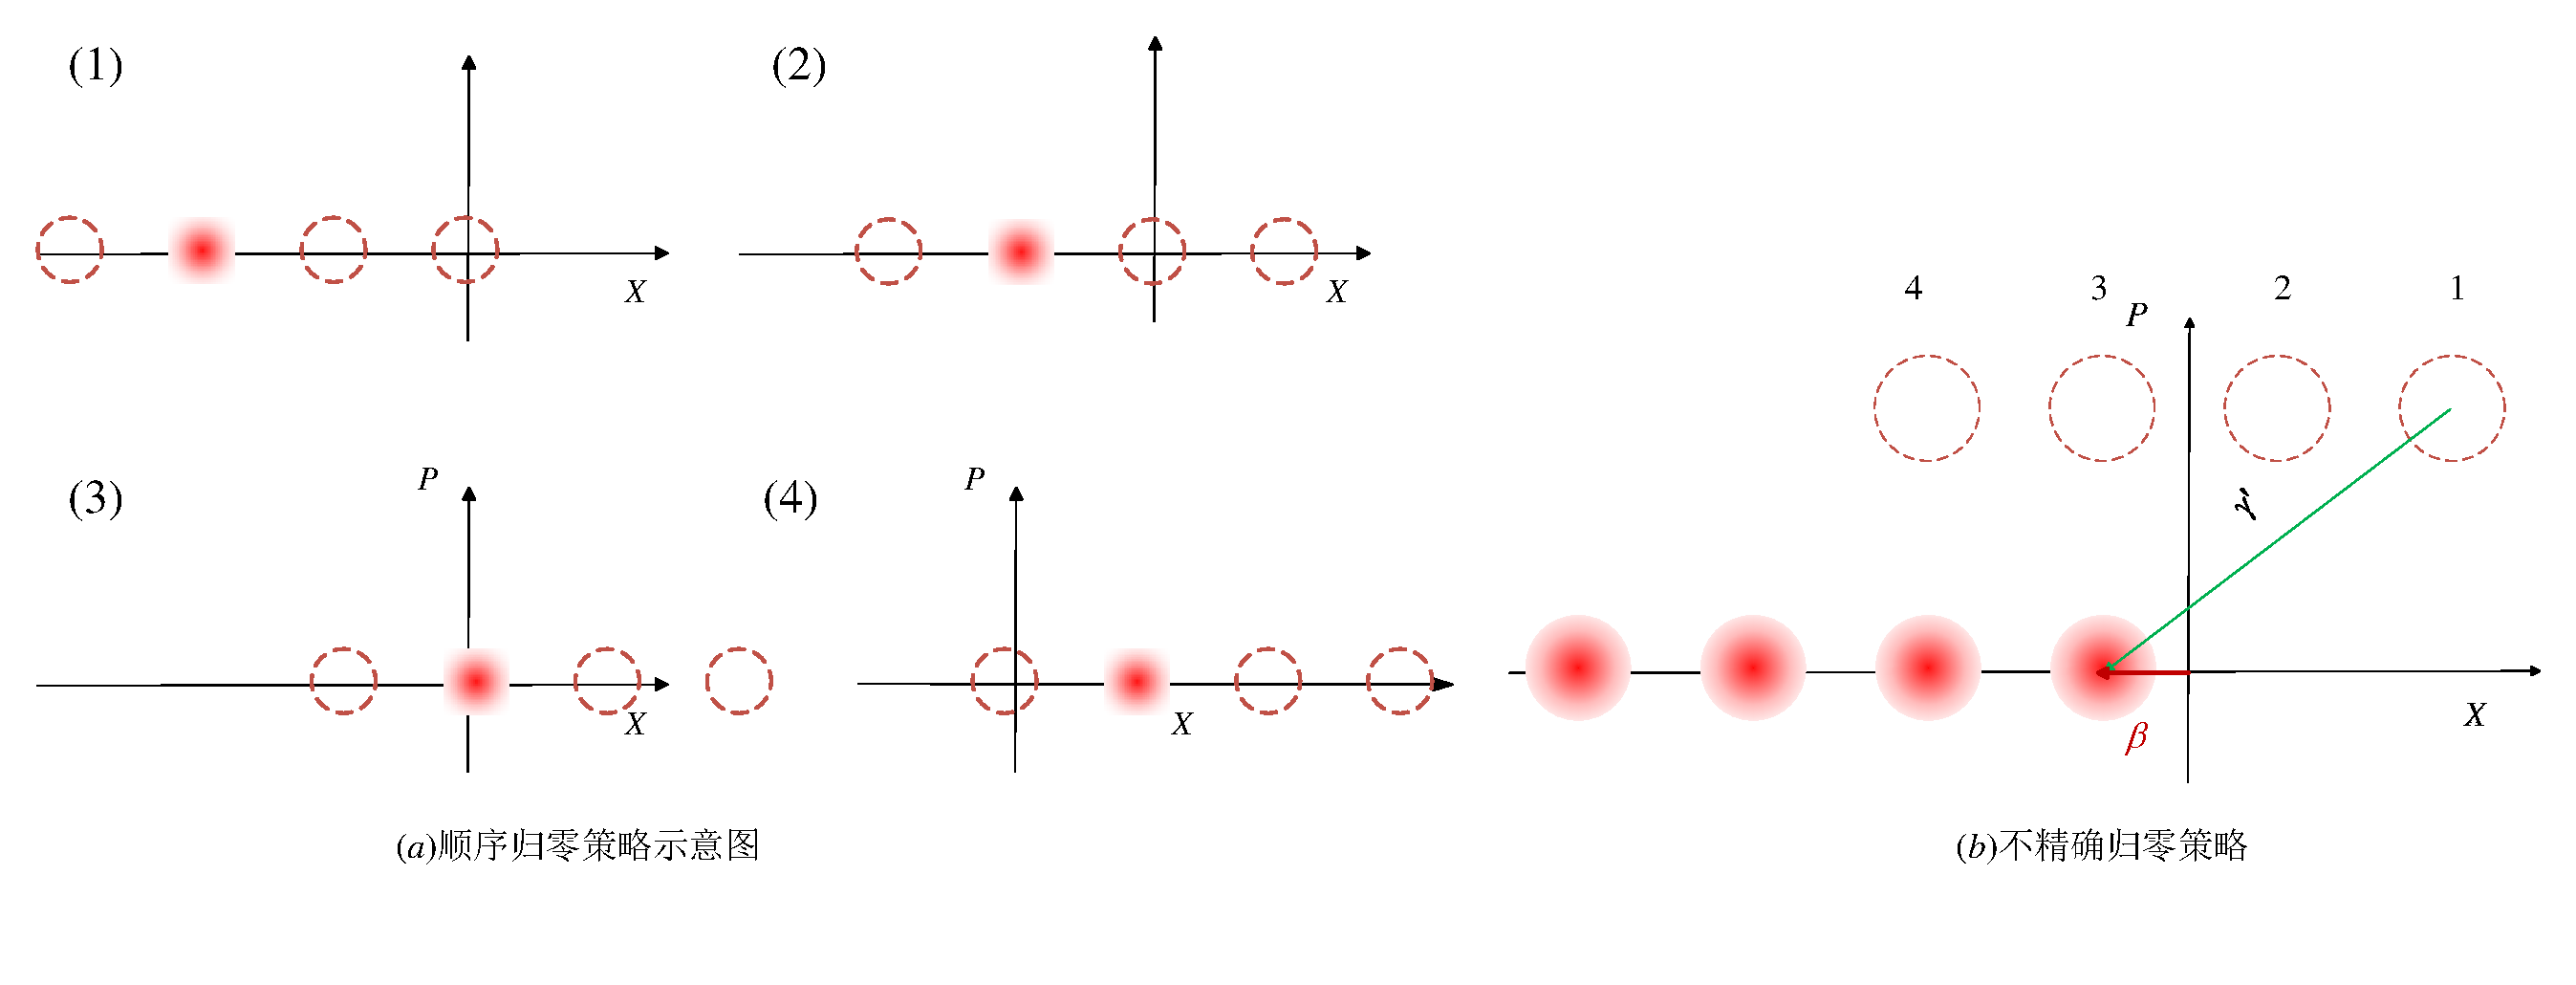
\includegraphics[width=\textwidth]{figures/chap3/Q-Bondurant-displacemet-strategy}
  \caption{四态区分的Bondurant接收机接收策略和不精确归零策略示意图}
  \label{fig:Q-Bondurant-displacemet-strategy}
\end{figure}

按照上述策略,
该$L$态区分的Bondurant接收机
的条件概率可以通过\ref{eq:QAM-cond-prob}式计算得到。
具体而言对信号$\alpha_{uv}$有
\begin{equation}
\begin{split}
P^{DR}\{u|\alpha_{uv}\} = & \int_0^1 dt_1 n_{u,1} e^{n_{u,1} t_1} \int_{t_1}^1 dt_2 n_{u,2} e^{n_{u,2} (t_2-t_1)}   \\
                          &\qquad \cdots \int_{t_{k-2}}^1 dt_{k-1} n_{u,k-1} e^{n_{u,k-1} (t_{k-1}-t_{k-2})}, u \in \Omega.
\end{split}
\label{eq:DR-cond-p}
\end{equation}
这里我们将时间对符号周期进行归一化了,
其中$k$为信号$\alpha_{uv}$探测正确时,
符号周期结束时刻接收机对应的归零符号序数,
满足$v = (L-1) - 2k$,且正确探测时,发生的光子计数事件数目为$k-1$个。
上式中$n_{v,i} = 4t^2|\alpha(k-i)|^2 $,
这里$t = \sqrt{T}$。

利用Bondurant接收机的渐近性能,注意到
$n_{v,i} \neq n_{v,l} $
对所有的$i \neq l$成立,所以
可得当光子数很大时
\begin{equation}
P_c^{DR} \approx 1 - C e^{-4t^2\alpha^2}.
\label{eq:QAM-Hybrid-approx-2}
\end{equation}

所以,两个接收机联合探测的正确概率为
\begin{equation}
\begin{split}
P_c &= \frac{1}{M} \sum_{u,v} P^{HD}\{v| \alpha_{uv}\} P^{DR}\{u|\alpha_{uv}\} \\
    &= \frac{1}{M} \sum_v P^{HD}\{v| \alpha_{uv}\} \sum_u P^{DR}\{u|\alpha_{uv}\} \\
    &= \left( \frac{1}{L} \sum_v P^{HD}\{v| \alpha_{uv}\} \right) \left( \frac{1}{L} \sum_u P^{DR}\{u|\alpha_{uv}\} \right) \\
    &= P_c^{HD} P_c^{DR}.
\end{split}
\end{equation}
这里$P_c^{HD}$和$P_c^{DR}$分别是
零差接收机平均正确探测概率和Bondurant接收机的平均正确探测概率。
当光子数很大时,利用式\ref{eq:QAM-Hybrid-approx-1}和\ref{eq:QAM-Hybrid-approx-2}
可得这种混合接收机的平均错误概率渐近性能为
\begin{equation}
\begin{split}
P_e & \approx \left(1 - (1-\frac{1}{L}) e^{-2r^2\alpha^2} \right) \left( 1 - C e^{-4t^2\alpha^2} \right)  \\
    & \approx (1-\frac{1}{L}) e^{-2r^2\alpha^2} +C e^{-4t^2\alpha^2} .
\end{split}
\end{equation}
如果取50:50的分束器,即$r^2 = t^2 = 0.5$,
那么
\begin{equation}
\begin{split}
P_e & \approx (1-\frac{1}{L}) e^{-\alpha^2}  .
\end{split}
\end{equation}
与经典外差接收机\ref{eq:QAM-SQL-approx}式相比,
这种混合接收机性能低3dB。
容易看到,当$2r^2 = 4t^2$时,具有最佳的渐近性能,
此时$r^2 = 2 t^2 = 2/3$,即需要采用一个反射率为$2/3$
的分束器,此时最佳渐进性能为
\begin{equation}
P_e \approx (1-\frac{1}{L}+C) e^{-\frac{4}{3}\alpha^2}  .
\end{equation}
与经典外差接收机\ref{eq:QAM-SQL-approx}式相比,
在大信号的时候,这种接收机具有指数倍的增益。




正如最优位移接收机那样,我们也可以在Bondurant接收机位移操作时,
采用不精确归零如图\ref{fig:Q-Bondurant-displacemet-strategy}(\textit{b})所示。
由于采用不精确归零,所以对于M阶QAM信号,
存在一定概率发生$L$个甚至超过$L$个光子计数事件,
在这种策略当中,我们将这种情形都判定为第$L$个符号。
假定这个附加的位移量恒定为$\beta$,那么对应的条件概率为
\begin{equation}
\begin{split}
P^{DR}\{u|\alpha_{uv}\} = & \int_0^1 dt_1 n_{u,1} e^{n_{u,1} t_1} \int_{t_1}^1 dt_2 n_{u,2} e^{n_{u,2} (t_2-t_1)} \\
                          & \cdots \int_{t_{k-2}}^1 dt_{k-1} n_{u,k-1} e^{n_{u,k-1} (t_{k-1}-t_{k-2})} \left( e^{n_{u,k} (1-t_{k-1})}\right), \\
                          & \qquad \qquad u \in \Omega \text{且} u \neq -(L-1);   \\
P^{DR}\{u|\alpha_{uv}\} = & \int_0^1 dt_1 n_{u,1} e^{n_{u,1} t_1} \int_{t_1}^1 dt_2 n_{u,2} e^{n_{u,2} (t_2-t_1)} \\
                          & \cdots \int_{t_{k-3}}^1 dt_{k-2} n_{u,k-2} e^{n_{u,k-2} (t_{k-2}-t_{k-3})} \left( 1 - e^{n_{u,k-1} (1-t_{k-2})}\right),  \\
                          & \qquad \qquad u = -(L-1).
\end{split}
\label{eq:DR-cond-p-2}
\end{equation}
在这里$n_{v,i} = 4r^2|\alpha(k-i)|^2 + |\beta|^2$是存在附加位移量时实际的平均光子数。
为了得到最优的附加位移量$\beta$,我们对$P^{DR}$进行数值优化,
\begin{equation}
\beta^* = \arg\max_{\beta} P^{DR}(\beta).
\end{equation}

\begin{figure}
\centering
  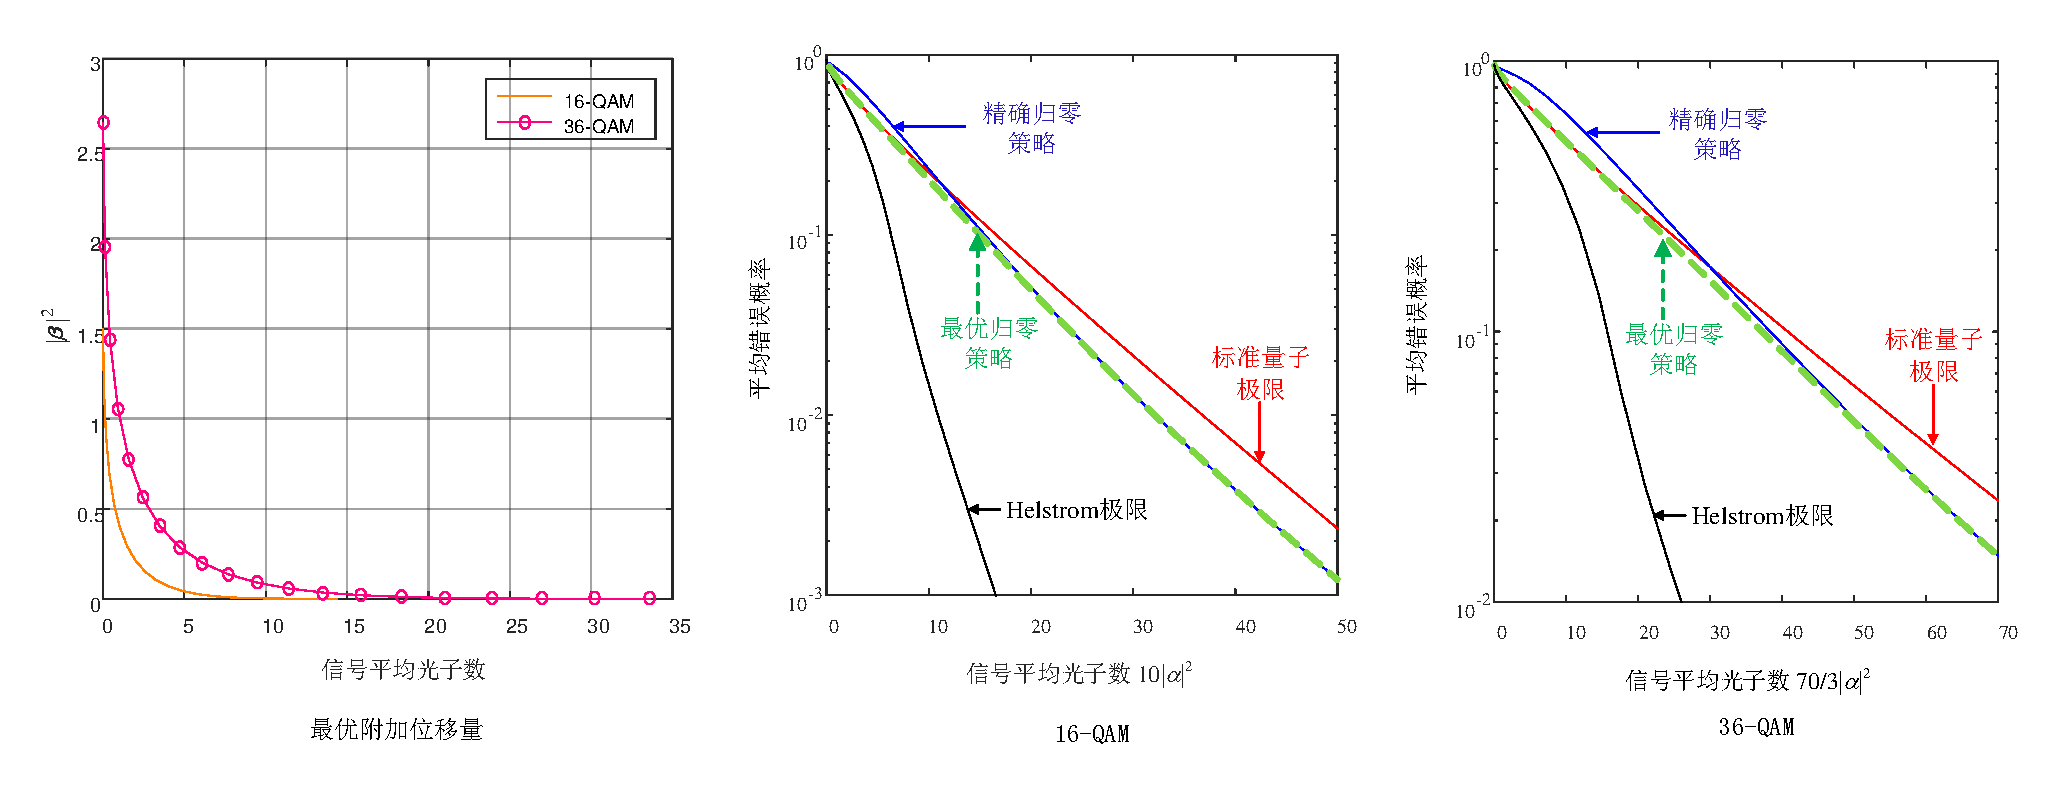
\includegraphics[width=\textwidth]{figures/chap3/QAM-Hybrid-error}
  \caption{QAM信号混合接收机性能}
  \label{fig:QAM-Hybrid-error}
\end{figure}


我们对16-QAM信号和36-QAM信号进行数值仿真,
透过率取$t^2=0.5$,
仿真结果如\ref{fig:QAM-Hybrid-error}图所示,可以看到随着光子数的增大,
两种策略都能突破标准量子极限,但是采用精确归零策略的接收机,
在小信号时性能比较差,而不精确归零策略则可以改善小信号时接收机的性能。
并且,随着光子数的增大,附加位移量迅速减小,
因此不精确归零策略的混合接收机渐近性能与精确归零一致。






\section{总结}

\begin{figure}
\centering
  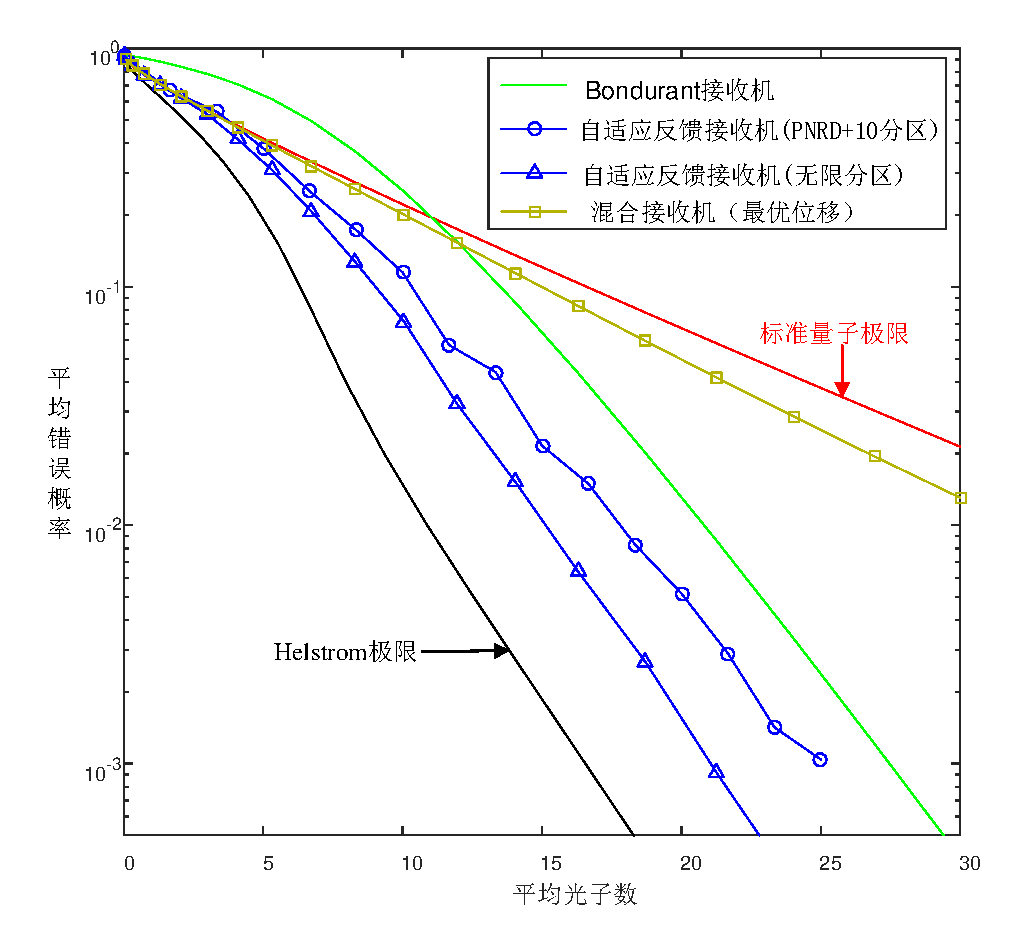
\includegraphics[width=0.6\textwidth]{figures/chap3/QAM-error}
  \caption{QAM信号三种接收机性能对比}
  \label{fig:QAM-error}
\end{figure}

在这一章,我们系统地分析了三种QAM信号量子接收机方案,
Bondurant接收机、自适应分区检测接收机以及混合接收机,
图\ref{fig:QAM-error}显示对于16-QAM信号,这三种接收机性能的一个对比。
首先,这三种接收机在光子数较大的时候都能突破标准量子极限,
Bondurant接收机在小信号的时候性能很差,混合接收机通过
最优位移策略改善了小信号时的性能。
其次,混合接收机性能最差,通过前面分析可知,
如果透过率为0.5,
那么其大信号渐近平均错误概率与标准量子极限仅相差3dB,
而另外两种接收机都比标准量子极限低一个指数项,
也就是具有指数倍的增益。
即使在最佳透过率的情况下,
接收性能还是不如另外两种接收策略,
由于对于高阶调制,采用混合接收机所减少的资源消耗
很少,因此对于QAM调制信号,不建议采用混合接收机进行探测。
最后,通过自适应分区检测的方法,
Bondurant接收机需要实时反馈控制以及小信号时的缺陷
都被解决了,因此自适应分区检测接收机具有非常高
的实用价值,并且通过前面的理论分析,
它的大信号渐近性能与Helstrom极限非常接近,
可以认为它是一种可实用化的近最优检测方案。





通过对现有的量子接收机的观察,
我们可以发现,对本振的反馈控制策略是导致接收机最终性能的关键。
在我们的分析中,Bondurant接收在两个光子到达的时间间隔期间,
采用恒定的位移量,而当一个光子到达探测器的时候,
立即调整本振。自适应分区检测接收在每一个分区,
也采用的是恒定的位移量。因此,如果不采用恒定的位移量,
而是随时间变化的位移量,能否找到这样一种最优的控制策略
是一个数学难题。
到目前为止,Dolinar接收机解决了二元信号的最优控制策略问题,
令人惊喜的是这种最优控制策略给出了最优量子检测的接收性能。
但是对于更高阶的问题,如QPSK、QAM信号,这个数学难题
尚未解决,需要进一步的研究工作。
另外,这种最优控制策略是否能够达到Helstrom极限也不不知道,
如果最优控制策略不能达到这个极限,
那么对于高阶调制信号,如何设计接收机使得接收性能达到Helstrom
极限也是一个有待研究的问题。
